% !TeX root = thesis.tex

\chapter{State of the Art}\label{chap:sota}

This chapter reviews the theoretical foundations and the current state of the art relevant to this dissertation. It begins by introducing the fundamental 
concepts of artificial intelligence, machine learning, and deep learning, providing the background required to understand the methodologies adopted in this work. 
It then discusses the main industrial monitoring and maintenance strategies, namely anomaly detection, fault detection, and predictive maintenance. Finally, the 
chapter reviews the most relevant literature on deep learning for industrial time-series analysis and multi-task learning, highlighting the research gap addressed 
by this dissertation.


\section{What is an AI System?} \label{sec:artificialinteligence}

Before reviewing the state of the art related to this dissertation, it is first necessary to define what constitutes an AI system.

According to the AI Act Regulation (EU) 2024/1689 of the European Parliament (\cite{European2025}), 
we can define an AI system as a system that is machine-based, can operate with some degree of autonomy,
may show signs of adaptiveness after its deployment, and from a given input it receives, 
generates an output that can influence its environment. These outputs can be predictions, 
content, recommendations, or decisions.

From an academic perspective, \cite{Russell2016} define AI in terms of 
intelligent agents, describing them as systems that perceive their environment through sensors and 
act upon that environment through actuators. Under this view, an AI system can be regarded 
as a function that maps observations of the environment to actions intended to achieve specific goals.

Although these definitions originate from different contexts, they share the same fundamental principle: an AI system receives information from its environment, processes it, 
and generates outputs intended to achieve one or more predefined objectives.

\section{Machine Learning} \label{sec:ml}

As discussed, AI systems are designed to perceive their environment, process information, and produce outputs depending on their objective. However, AI is a broad field that encompasses a wide range of techniques, from 
rule-based systems to modern data-driven approaches (\cite{Russell2016}).

ML is one of the most important branches of AI. Rather than relying on explicitly programmed rules, ML enables computers to automatically learn patterns and relationships from data, allowing them to improve their performance on 
a given task through experience. This paradigm has become the dominant approach to AI in recent decades due to the increasing availability of large datasets and advances in computational resources (\cite{Mitchell2013,Goodfellow2016}).

According to Mitchell \cite{Mitchell2013}, \emph{"a computer program is said to learn from experience $E$ with respect to some class of tasks $T$ and performance measure $P$, if its performance at tasks in $T$, as measured by $P$, 
improves with experience $E$."} This definition emphasizes that learning is not achieved by explicitly programming every possible decision, but rather by allowing the algorithm to discover useful patterns directly from data.

Today, ML constitutes the foundation of most modern AI systems. Depending on the complexity of the task and the amount of available data, different learning algorithms can be employed, ranging from traditional 
statistical methods to deep neural networks. The following sections introduce the main ML paradigms and describe the typical workflow followed during the development of ML models.

\subsection{ML Paradigms} \label{sec:mlpara}

Machine learning algorithms can be broadly categorized according to the information available during training. The four main learning paradigms are supervised learning, unsupervised learning, reinforcement learning, 
and self-supervised learning. Although they share the common objective of extracting useful information from data, they differ in the learning signal available to the algorithm, the optimization objective, and the types of 
tasks they are designed to solve (\cite{Murphy2022}).

\subsubsection{Supervised Learning}

Supervised learning is the most widely adopted machine learning paradigm and is used when a dataset contains both the input variables, commonly referred to as \textit{features}, \textit{covariates}, or \textit{predictors}, and 
their corresponding desired outputs, known as \textit{labels}. The goal is to learn a mapping between the input variables and the corresponding output so that the model can accurately predict the labels of previously unseen 
observations \cite{Murphy2022}.

Depending on the nature of the target variable, supervised learning problems are generally divided into two main categories. When the target variable belongs to a finite set of discrete classes, the problem is known 
as \textit{classification}. Typical applications include fault diagnosis, image recognition, and spam detection. Conversely, when the target variable is continuous, the problem is referred to as \textit{regression}, where the 
objective is to predict numerical quantities such as energy consumption, or product demand.

Table~\ref{tab:supervised_dataset} presents an example of a supervised learning dataset. Each observation contains four input features describing the physical characteristics of an Iris flower, together with the corresponding 
species label. The objective is to learn a model capable of predicting the flower species (Figure~\ref{fig:iris_flowers}) from the measured features.

\begin{table}[htbp]
\centering
\caption{Example of the Iris dataset used for supervised classification. Adapted from \cite{Murphy2022}}
\label{tab:supervised_dataset}

\begin{tabular}{cccccc}
\toprule
\textbf{index} & \textbf{Sepal Length} & \textbf{Sepal Width} & \textbf{Petal Length} & \textbf{Petal Width} & \textbf{label} \\
\midrule
0   & 5.1 & 3.5 & 1.4 & 0.2 & Setosa \\
1   & 4.9 & 3.0 & 1.4 & 0.2 & Setosa \\
$\vdots$ & $\vdots$ & $\vdots$ & $\vdots$ & $\vdots$ & $\vdots$ \\
50  & 7.0 & 3.2 & 4.7 & 1.4 & Versicolor \\
$\vdots$ & $\vdots$ & $\vdots$ & $\vdots$ & $\vdots$ & $\vdots$ \\
149 & 5.9 & 3.0 & 5.1 & 1.8 & Virginica \\
\bottomrule
\end{tabular}

\end{table}

\begin{figure}[htbp]
    \centering
    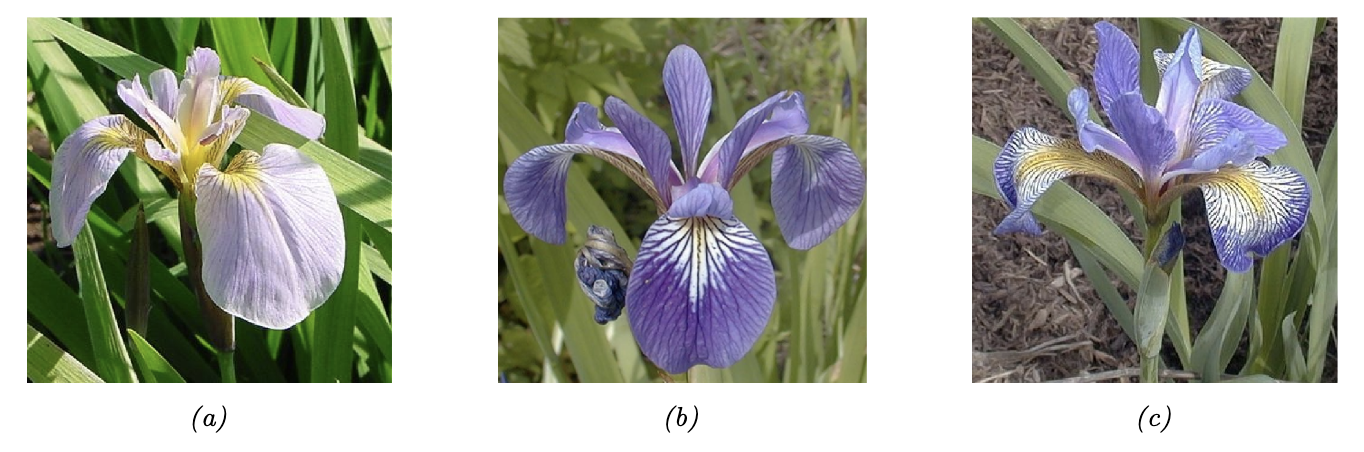
\includegraphics[width=0.80\textwidth]{imgs/iris flowers.png}
    \caption{Three types of Iris flowers: Setosa, Versicolor and Virginica. Adapted from \cite{Murphy2022}}
    \label{fig:iris_flowers}
\end{figure}

In the context of our work, supervised learning is commonly employed for tasks such as AD, FC and PdM, where historical operational data together with fault labels or degradation measurements are available.

\subsubsection{Unsupervised Learning}

Unlike supervised learning, unsupervised learning does not deal with datasets that contain labels. Consequently, the learning algorithm must discover patterns, structures, relationships  or other type of useful information
directly from the data without being provided with the desired output (\cite{Murphy2022}).

Common unsupervised learning tasks include \textit{clustering}, where similar observations are grouped according to their characteristics, \textit{dimensionality reduction}, which aims to represent high-dimensional data using a smaller number of informative 
variables, and \textit{density estimation}, which models the probability distribution of the data.

\subsubsection{Reinforcement Learning}

Reinforcement learning addresses sequential decision-making problems, where an intelligent agent learns by interacting with an environment rather than from a fixed 
dataset (\cite{Murphy2022}). At each time step, the agent observes the current state of the environment, selects an action according to its policy, and receives a numerical reward indicating the quality of the chosen action. 
Based on this interaction, the environment transitions to a new state, and the process is repeated.

The objective of reinforcement learning is to learn an optimal policy that maximizes the expected cumulative reward over time. Since the consequences of an action may only become apparent after several subsequent decisions, the 
agent must balance \textit{exploration}, by trying new actions to acquire knowledge about the environment, and \textit{exploitation}, by selecting the actions that are currently believed to yield the highest reward.

Figure~\ref{fig:reinforcement_learning} illustrates the reinforcement learning framework. The agent continuously interacts with the environment by observing its current state, 
selecting an action, and receiving both a reward and the next state. Through this trial-and-error process, the agent gradually learns a policy that maximizes the expected cumulative 
reward.

\begin{figure}[htbp]
    \centering
    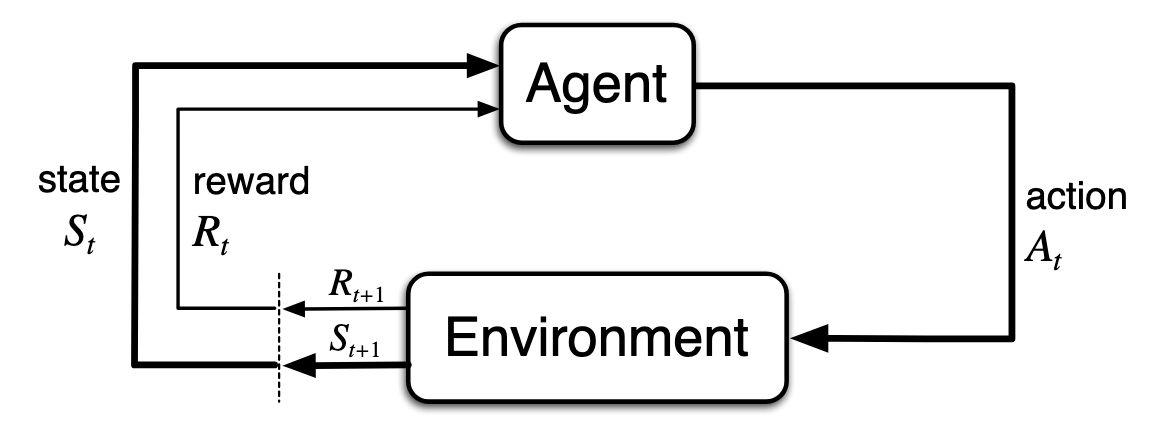
\includegraphics[width=0.80\textwidth]{imgs/reinforcement_learning.png}
    \caption{Agent–environment interaction in reinforcement learning. Adapted from \cite{Sutton2018}}
    \label{fig:reinforcement_learning}
\end{figure}

\subsubsection{Self-Supervised Learning}

Self-supervised learning is a learning paradigm in which supervision is obtained directly from the data itself rather than from manually annotated labels (\cite{Murphy2022}). Instead of relying on external ground-truth 
annotations, the learning algorithm constructs auxiliary or \textit{pretext} tasks whose targets are automatically generated from the input data. By solving these tasks, the model learns meaningful representations that capture 
the underlying structure of the data.

In recent years, self-supervised learning has become one of the most active research areas in machine learning, achieving remarkable success in computer vision, natural language processing and speech processing.

\subsection{Representation Learning} \label{sec:rep_l}

The machine learning paradigms presented in the previous section describe the different ways in which models can learn from data. Regardless of the learning 
paradigm, the performance of a machine learning algorithm largely depends on the quality of the data representation used to describe the problem.

For relatively simple problems, carefully designed features may be sufficient to achieve good performance. For instance, if the objective is to distinguish 
between male and female speakers, a feature such as the average vocal tract length or the fundamental frequency may already provide enough information for a 
traditional classifier. However, many real-world problems involve highly complex and high-dimensional data, making it extremely difficult to manually define 
informative features. Image classification is a representative example of such complexity. A model cannot recognize an animal directly from the raw pixel values of an image. Instead, 
it must first learn simple representations, such as edges and textures, which are then combined to form higher-level features such as shapes, body parts, and 
eventually complete objects. This hierarchical learning process allows increasingly abstract representations to be constructed from simpler ones. This concept is called
representation learning (\cite{Goodfellow2016}). Figure~\ref{fig:dl_image} illustrates the concept of hierarchical representation learning.

\begin{figure}[htbp]
    \centering
    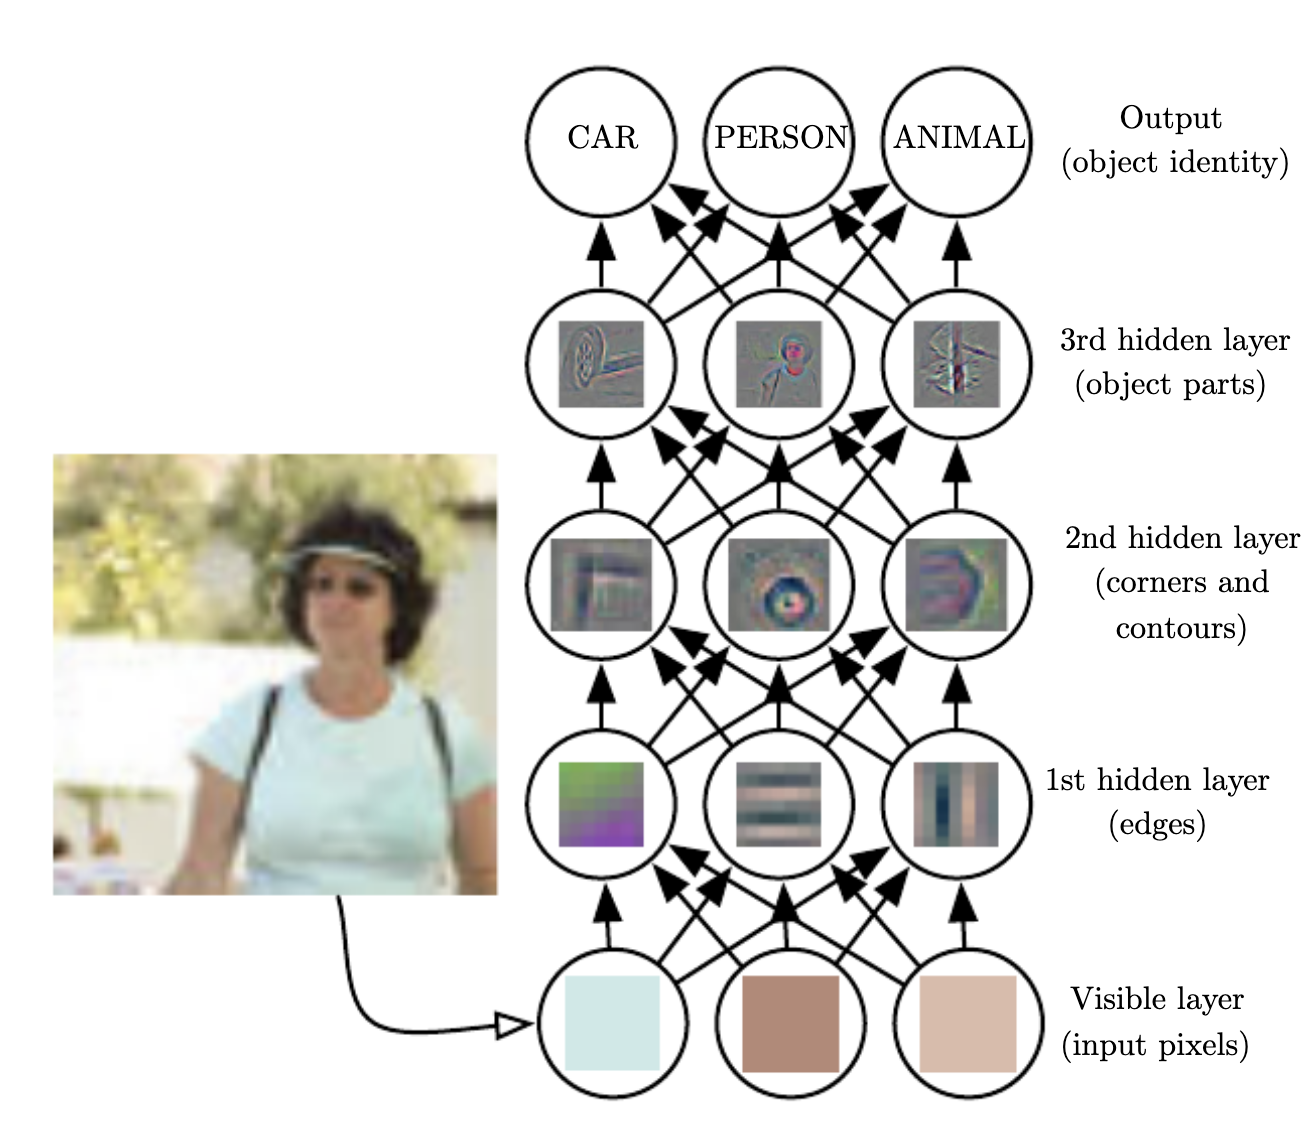
\includegraphics[width=0.80\textwidth]{imgs/dl_image.png}
    \caption{Illustration of a representation learning model. Adapted from \cite{Goodfellow2016}}
    \label{fig:dl_image}
\end{figure}

\subsection{Deep Learning} \label{sec:dl}

Representation learning provides the foundation for DL. Rather than relying on manually engineered features, DL algorithms automatically discover 
multiple levels of representation by composing a sequence of simple transformations. This hierarchical organization enables models to learn increasingly abstract 
features directly from raw data, making them particularly effective for solving complex tasks such as computer vision, speech recognition, and natural language 
processing (\cite{Goodfellow2016}).

Most modern DL models are implemented using Artificial Neural Networks (ANNs). These models are constructed by composing multiple layers of simple nonlinear 
transformations, allowing increasingly abstract representations of the input data to be learned automatically (\cite{Goodfellow2016}).

The following section introduces the fundamental concepts behind ANNs, which constitute the basis of most modern DL models.

\subsubsection{Artificial Neural Networks}

From a mathematical perspective, an ANN can be regarded as a parameterized function that maps an input vector $\mathbf{x}$ to an output $\mathbf{h}$. During 
training, the parameters of this function are optimized so that the network approximates the underlying relationship between the input data and the 
desired output (\cite{Goodfellow2016}).

The fundamental computational unit of an ANN is the artificial neuron, also known as a perceptron (\cite{Rosenblatt1958}). A perceptron receives one or more input 
variables, computes a weighted sum of these inputs, adds a bias term, and applies a nonlinear activation function to produce its output. Mathematically, this 
operation can be expressed as

\begin{equation}
h = g(\mathbf{w}^{T}\mathbf{x} + b)
\label{eq:neuron}
\end{equation}

where $\mathbf{x}$ denotes the input vector, $\mathbf{w}$ is the vector of trainable weights, $\mathbf{b}$ is the bias term, and $\mathbf{g}$ represents the activation 
function. Figure~\ref{fig:perceptron} illustrates the structure of a perceptron.

\begin{figure}[htbp]
    \centering
    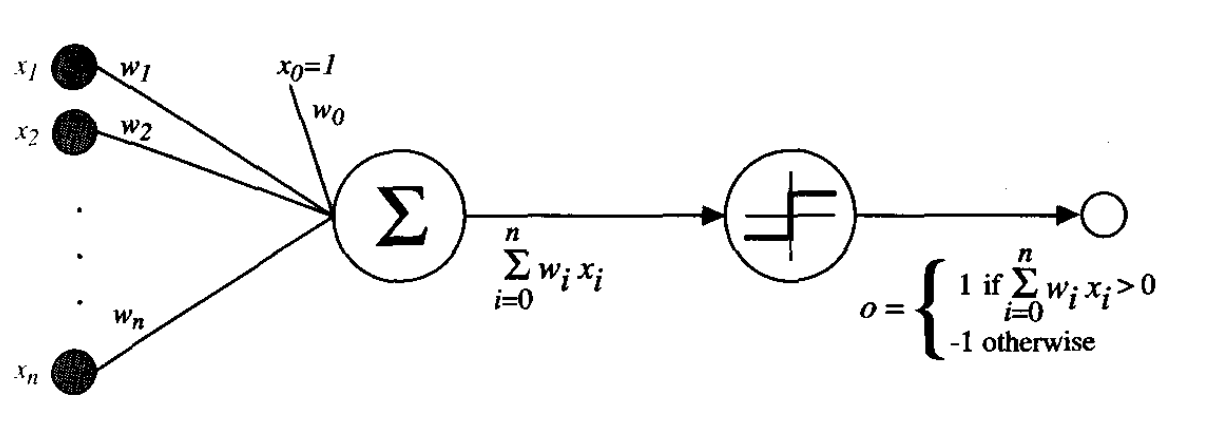
\includegraphics[width=0.80\textwidth]{imgs/perceptron.png}
    \caption{Illustration of a perceptron. Adapted from \cite{Mitchell2013}}
    \label{fig:perceptron}
\end{figure}

Although the perceptron constitutes the fundamental computational unit of an ANN, practical problems generally require much more expressive models. To achieve 
this, multiple perceptrons are interconnected and organized into successive layers, forming a feedforward neural network, commonly referred to as a Multilayer 
Perceptron (MLP). The network typically consists of an input layer, one or more hidden layers, and an output layer. Each neuron receives the outputs of the 
previous layer, performs the operation defined in Equation~\ref{eq:neuron}, and forwards its output to the next layer.

By stacking multiple hidden layers, an MLP is capable of learning increasingly abstract representations of the input data, allowing it to approximate highly 
complex nonlinear functions (\cite{Goodfellow2016}). Figure~\ref{fig:mlp} illustrates the general architecture of a Multilayer Perceptron.

\begin{figure}[htbp]
    \centering
    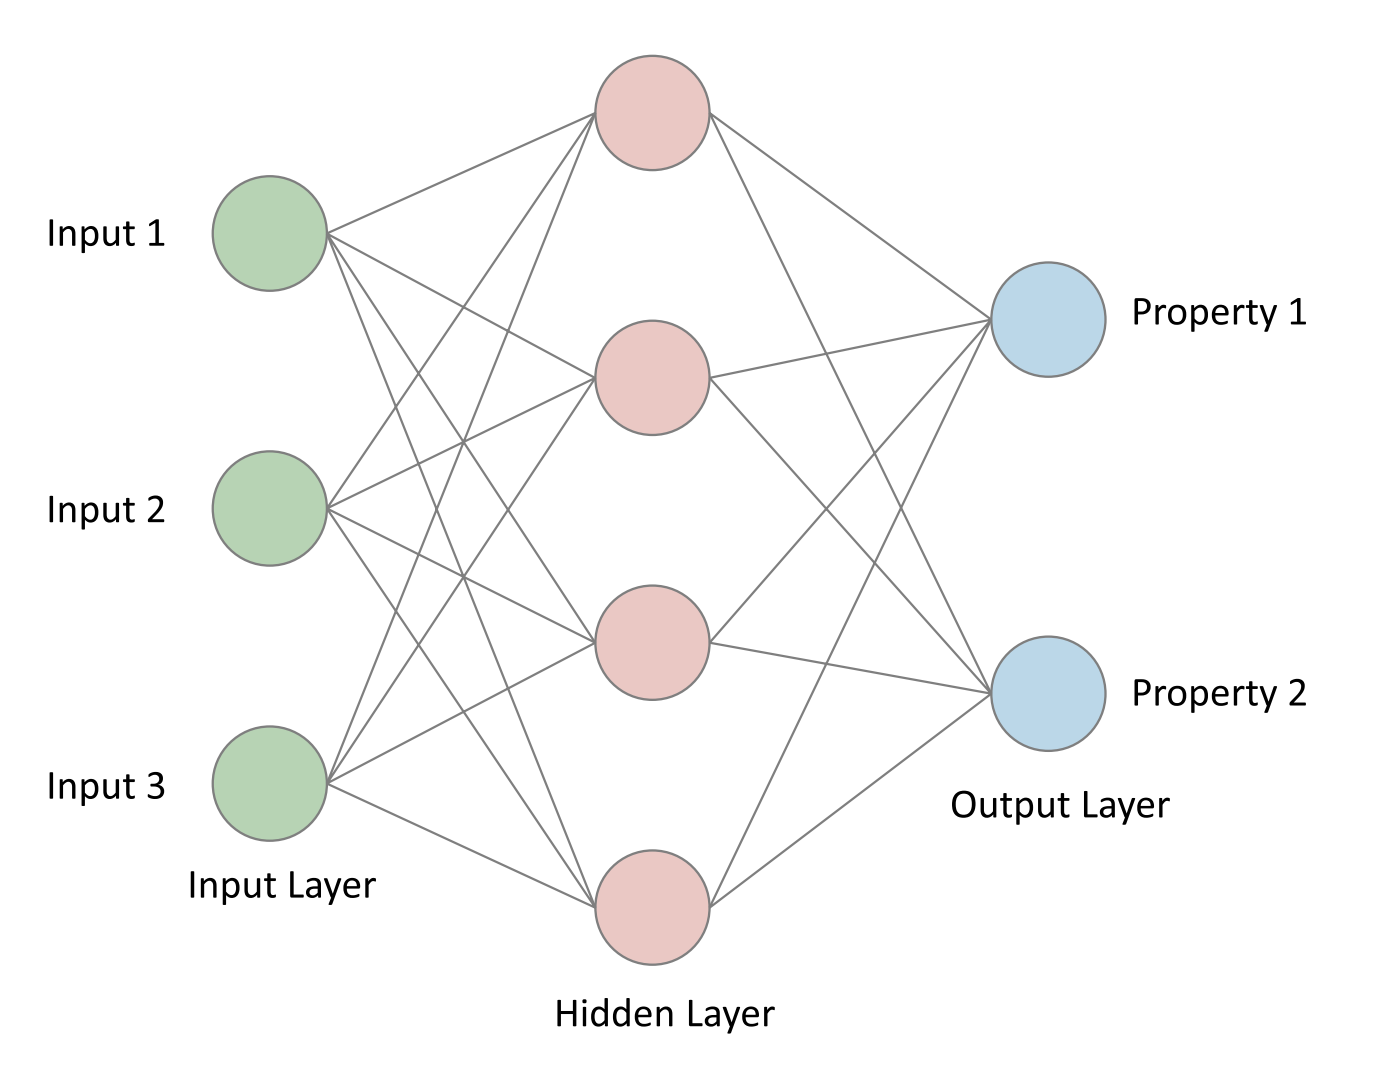
\includegraphics[width=0.80\textwidth]{imgs/mlp.png}
    \caption{Illustration of a MLP with 1 hidden layer. Adapted from \cite{Zhang2023}}
    \label{fig:mlp}
\end{figure}


\subsection{Training Deep Neural Networks} \label{sec:training}

Once the architecture of a neural network has been defined, the next step is to determine the values of its parameters, namely the weights and biases. This process, known as training, consists of finding the set of parameters
that minimizes a \emph{cost function} $J(\theta)$, defined as the average loss incurred by the model over the training set (\cite{Goodfellow2016}). During training, the network 
repeatedly processes examples from the training dataset, evaluates the quality of its predictions through a \emph{loss function}, and updates its parameters in order to reduce this cost.

In practice, the cost function is rarely evaluated over the entire training set at every update. Instead, most deep learning models are trained using \emph{stochastic gradient descent} (SGD) or one of its variants, in which 
the gradient is estimated from a small, randomly sampled \emph{mini-batch} of examples at each iteration. This trades off the accuracy of the gradient estimate for a substantial reduction in computational cost per update, and 
is essential for training on large datasets (\cite{Goodfellow2016}).

This optimization process can be divided into four main stages: forward propagation, loss (cost) computation, backpropagation, and parameter update. These four stages are repeated iteratively, 
over mini-batches and across multiple passes (epochs) over the training set, until the model converges or a predefined stopping criterion is reached (\cite{Goodfellow2016}).

\begin{figure}[htbp]
\centering

\begin{tikzpicture}[
    node distance=0.9cm,
    every node/.style={
        draw,
        rounded corners,
        minimum width=5.5cm,
        minimum height=0.8cm,
        align=center,
        font=\small
    },
    arrow/.style={
        -{Latex[length=2.5mm]},
        thick
    }
]

\node (input) {Mini-batch of Training Data};
\node (forward) [below=of input] {Forward Propagation};
\node (prediction) [below=of forward] {Prediction $\hat{y}$};
\node (loss) [below=of prediction] {Cost Function $J(\theta)$};
\node (backward) [below=of loss] {Backpropagation (Gradient $\nabla_\theta J$)};
\node (update) [below=of backward] {Parameter Update (SGD / Adam)};

\draw[arrow] (input) -- (forward);
\draw[arrow] (forward) -- (prediction);
\draw[arrow] (prediction) -- (loss);
\draw[arrow] (loss) -- (backward);
\draw[arrow] (backward) -- (update);

% Loop back
\draw[arrow] (update.east) -- ++(2,0)
                  |- (forward.east);

\end{tikzpicture}

\caption{General training pipeline of a deep neural network. Backpropagation computes the gradient of the cost function; the optimization rule (e.g., SGD or Adam) then uses this gradient to update the parameters.}
\label{fig:training_pipeline}

\end{figure}

\subsection{Deep Learning Architectures} \label{sec:dparqui}

Over the years, numerous deep learning architectures have been proposed to address different types of learning problems. Each architecture is designed to exploit specific characteristics of the input data and is therefore 
suited to different application domains.

Since this dissertation focuses on industrial time-series data, only the architectures that are directly relevant to this work are presented. In particular, this section introduces recurrent neural networks (RNNs) and their 
Long Short-Term Memory (LSTM) variant, which constitute the foundation of the models developed in the following chapters.

\subsubsection{Recurrent Neural Network} \label{sec:rnn}

Feedforward neural networks process each input independently, without retaining information from previous inputs. Consequently, they are unable to capture temporal dependencies that naturally arise in sequential data. 
Recurrent Neural Networks (RNNs) overcome this limitation by introducing recurrent connections that allow information from previous time steps to be propagated through the network.

Unlike feedforward networks, an RNN maintains an internal hidden state that acts as a memory of past observations. At each time step, the hidden state is updated using both the current input and the hidden state from the 
previous time step. This enables the network to exploit temporal dependencies when making predictions (\cite{Goodfellow2016}).

\begin{equation}
\mathbf{h}_t = g(\mathbf{W}_{xh}\mathbf{x}_t + \mathbf{W}_{hh}\mathbf{h}_{t-1} + \mathbf{b})
\label{eq:rnn}
\end{equation}

Figure~\ref{fig:rnn} illustrates the recurrent structure of an RNN unfolded through time. The same set of parameters is shared across all time steps, allowing the network to process sequences of arbitrary length while 
maintaining information from previous observations.

\begin{figure}[htbp]
    \centering
    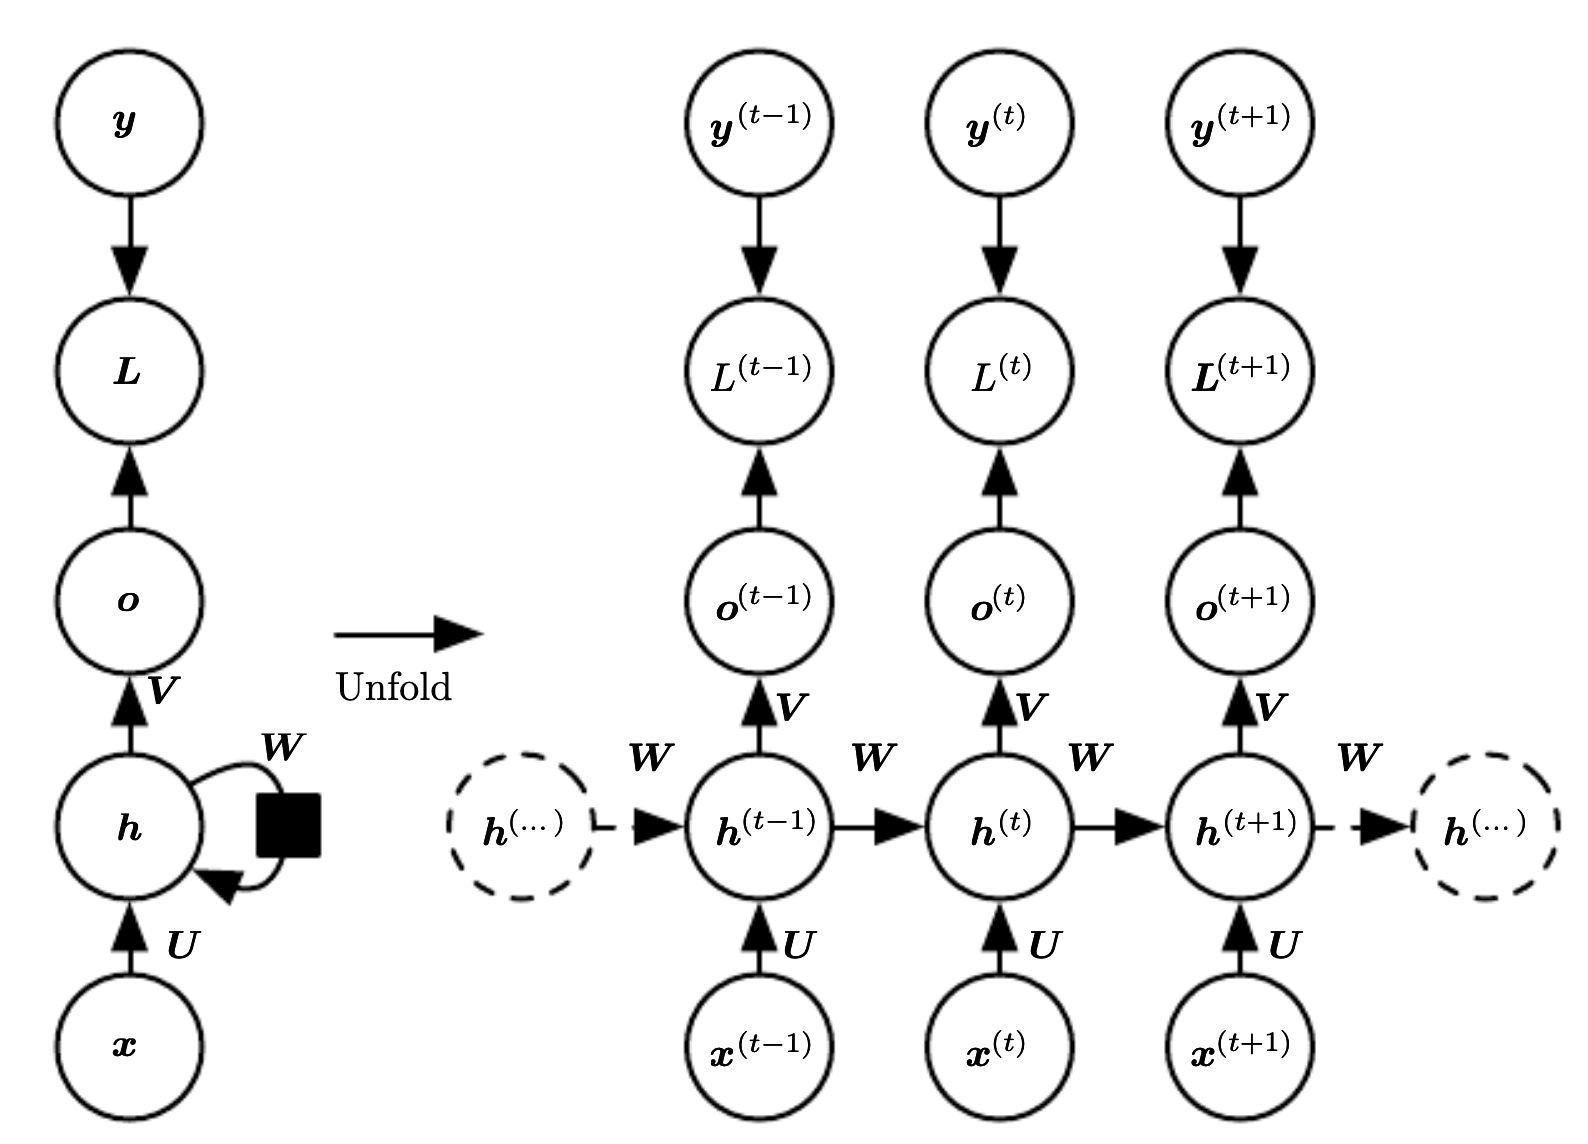
\includegraphics[width=0.80\textwidth]{imgs/rnn.png}
    \caption{Illustration of a RNN. Adapted from \cite{Goodfellow2016}}
    \label{fig:rnn}
\end{figure}

Although RNNs are theoretically capable of modeling long-term dependencies, in practice they suffer from the vanishing and exploding gradient problems during training. As a consequence, learning information over long sequences 
becomes difficult. To address this limitation, the Long Short-Term Memory (LSTM) architecture was proposed (\cite{Hochreiter1997}).

\subsubsection{Long Short-Term Memory} \label{sec:lstm}

Long Short-Term Memory (LSTM) networks were proposed by Hochreiter and Schmidhuber in 1997 to overcome the limitations of conventional RNNs when modeling long-term dependencies (\cite{Hochreiter1997}). Unlike a standard RNN, an 
LSTM introduces a memory cell that is specifically designed to preserve relevant information over long sequences while discarding irrelevant information.

The key component of an LSTM is its gating mechanism, which regulates the flow of information through the network. Three gates are responsible for this process: the forget gate determines which information from the previous 
memory should be discarded, the input gate decides which new information should be stored in the memory cell, and the output gate controls which information is propagated to the hidden state and the subsequent time step. By 
explicitly controlling the information flow, LSTMs mitigate the vanishing gradient problem and are therefore capable of learning much longer temporal dependencies than conventional RNNs (\cite{Goodfellow2016}).

Figure~\ref{fig:lstm} illustrates the internal structure of an LSTM cell. At each time step, the forget, input, and output gates regulate the information stored in the cell state, allowing the network to selectively retain or 
discard information according to its relevance for future predictions.

\begin{figure}[htbp]
    \centering
    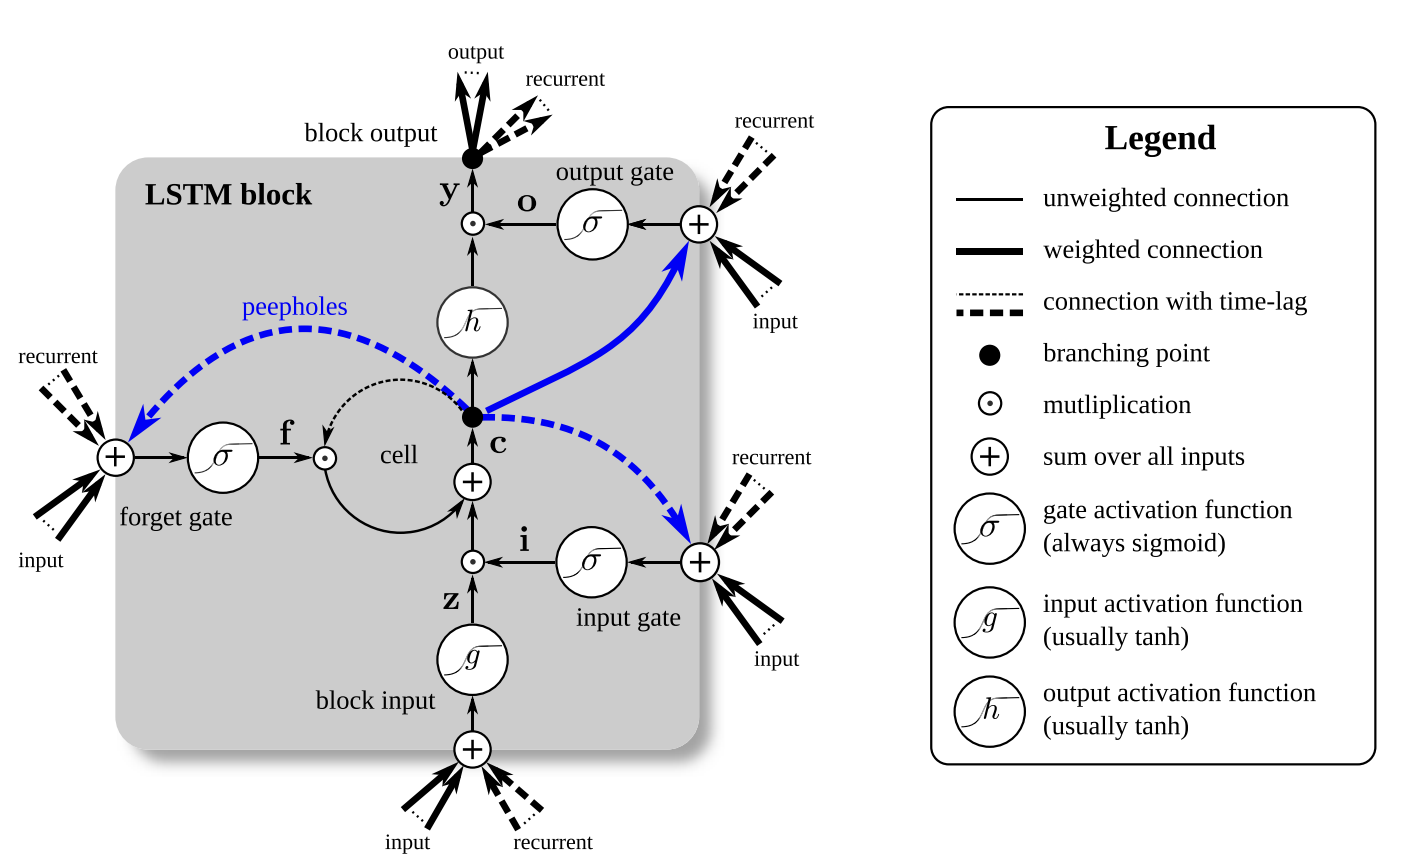
\includegraphics[width=0.80\textwidth]{imgs/lstm.png}
    \caption{Illustration of a LSTM. Adapted from \cite{Greff2017}}
    \label{fig:lstm}
\end{figure}

\subsection{Learning Strategies} \label{sec:learning_strategies}

The architectures presented in the previous sections describe how neural networks process information. However, the same architecture can be trained following different learning strategies depending on the number of tasks the 
model is expected to perform. The two most common approaches are single-task learning and multi-task learning (\cite{Zhang2022}).

In single-task learning (STL), a model is trained to perform only one prediction task by optimizing a single objective function. As a result, a separate model must be developed and trained for each task of interest. In contrast, 
multi-task learning (MTL) trains a single model to perform multiple related tasks simultaneously. This is typically achieved by sharing part of the network among all tasks while using task-specific output layers. By learning a
shared representation, MTL can exploit the common information between related tasks, often leading to improved generalization, better data efficiency, and reduced overfitting when compared with training 
independent models (\cite{Zhang2022}).

Figure~\ref{fig:stl_mtl} illustrates the conceptual difference between the two learning strategies. While STL requires an independent model for each prediction task, MTL relies on a shared feature extraction stage followed by 
multiple task-specific output branches. Figure~\ref{fig:mtl_example} shows an example multi-task feedforward neural network.

\begin{figure}[htbp]
\centering
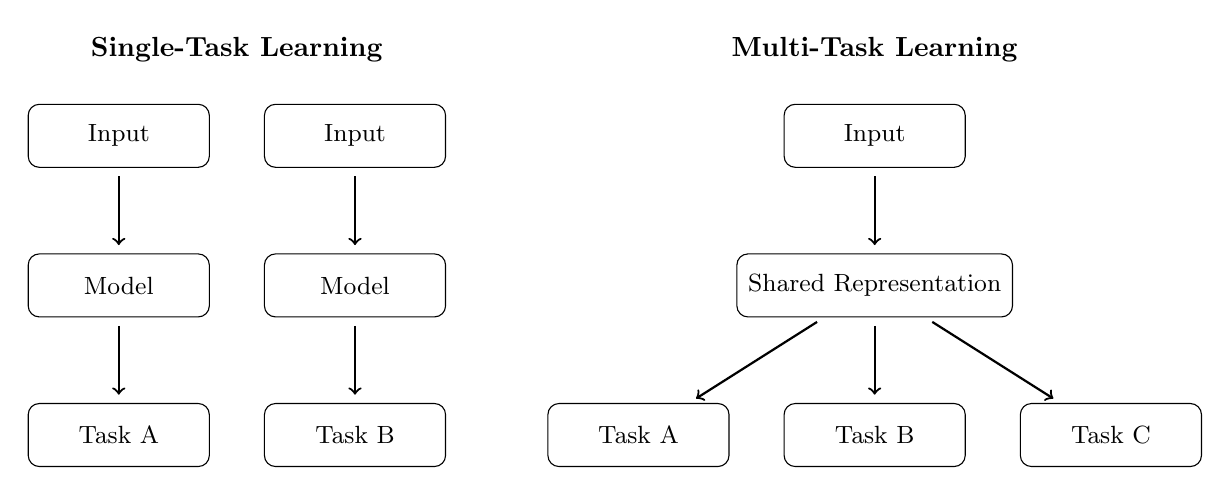
\begin{tikzpicture}[
    box/.style={
        draw,
        rounded corners,
        minimum width=2.3cm,
        minimum height=0.8cm,
        align=center,
        font=\small
    },
    arrow/.style={->, thick, shorten >=3pt, shorten <=3pt}
]
%==========================
% STL
%==========================
\node at (-3.5,3.0) {\textbf{Single-Task Learning}};

\node[box] (in1) at (-5,1.9) {Input};
\node[box] (m1)  at (-5,0)   {Model};
\node[box] (o1)  at (-5,-1.9){Task A};
\draw[arrow] (in1) -- (m1);
\draw[arrow] (m1) -- (o1);

\node[box] (in2) at (-2,1.9) {Input};
\node[box] (m2)  at (-2,0)   {Model};
\node[box] (o2)  at (-2,-1.9){Task B};
\draw[arrow] (in2) -- (m2);
\draw[arrow] (m2) -- (o2);

%==========================
% MTL
%==========================
\node at (4.6,3.0) {\textbf{Multi-Task Learning}};

\node[box] (input) at (4.6,1.9) {Input};
\node[box, minimum width=3.5cm] (shared) at (4.6,0)
{Shared Representation};
\node[box] (ta) at (1.6,-1.9) {Task A};
\node[box] (tb) at (4.6,-1.9) {Task B};
\node[box] (tc) at (7.6,-1.9) {Task C};

\draw[arrow] (input) -- (shared);
\draw[arrow] (shared) -- (ta);
\draw[arrow] (shared) -- (tb);
\draw[arrow] (shared) -- (tc);

\end{tikzpicture}
\caption{Conceptual comparison between single-task learning and multi-task learning. In STL, each task requires an independent model, whereas MTL shares a common representation across multiple related tasks while maintaining task-specific output layers.}
\label{fig:stl_mtl}
\end{figure}

\begin{figure}[htbp]
    \centering
    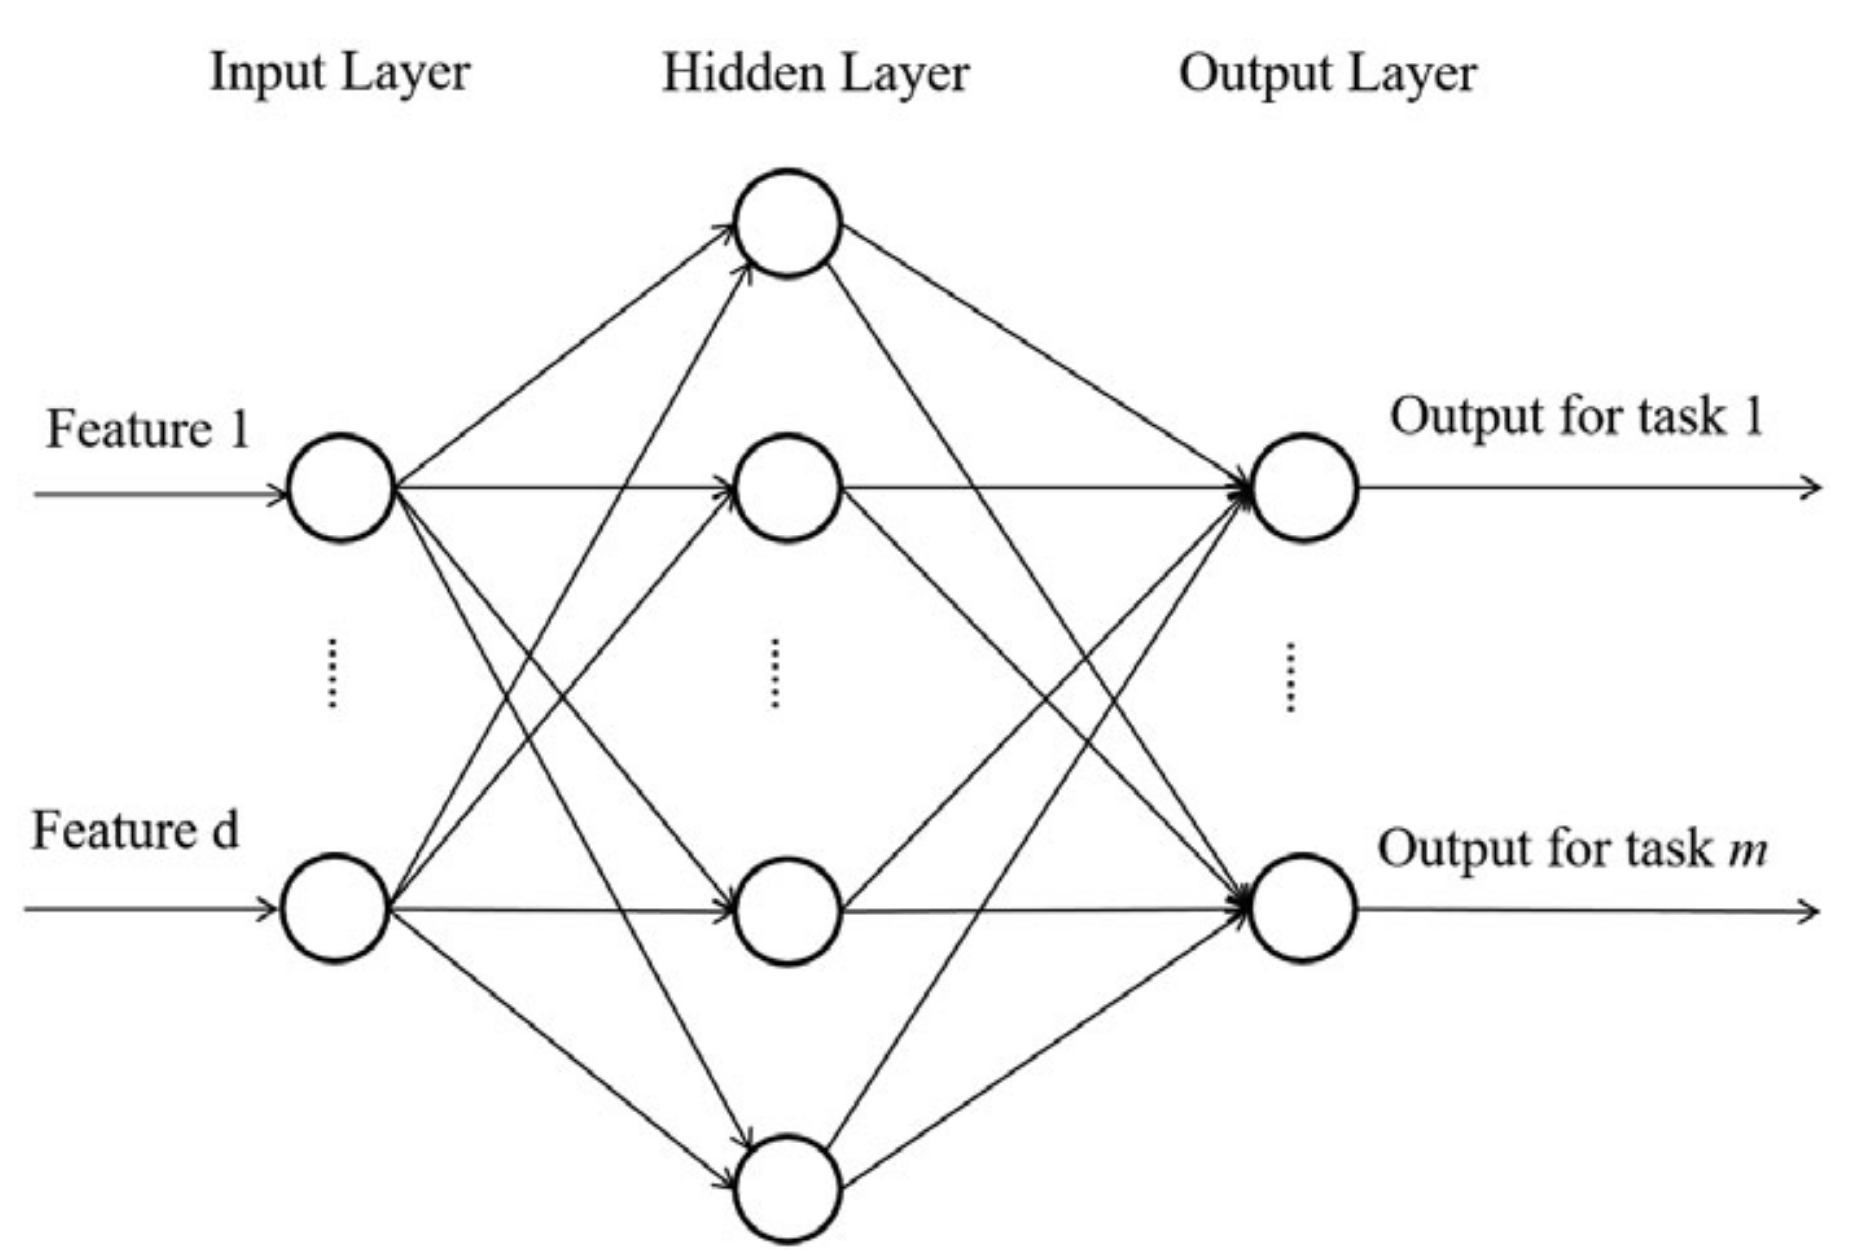
\includegraphics[width=0.80\textwidth]{imgs/mtl_example.png}
    \caption{Example for the multi-task feedforward neural network with an input layer, a hidden layer, and an output layer.. Adapted from \cite{Zhang2022}}
    \label{fig:mtl_example}
\end{figure}

\section{Industrial Monitoring and Maintenance} \label{sec:industrial_monitoring}

Modern industrial systems are increasingly equipped with a large number of sensors that continuously monitor the operating conditions of equipment and 
production processes. These sensors generate large volumes of operational data, including measurements of pressure, temperature, flow rate, vibration, 
electrical variables, and other process parameters. By analyzing these data, it is possible to assess the health of industrial assets, identify abnormal operating 
conditions, detect faults, and anticipate potential failures before they lead to unplanned downtime.

To support these objectives, several data-driven monitoring and maintenance strategies have been developed. Among the most widely adopted are anomaly 
detection (AD), fault detection (FD), and predictive maintenance (PdM). Although these concepts are closely related, they address different stages of the 
equipment health monitoring process and provide complementary information for supporting maintenance decisions. The following sections introduce each of these 
concepts and discuss their relationship.

\subsection{Anomaly Detection} \label{sec:ad}

Anomaly Detection (AD) is the process of identifying observations, events, or patterns that deviate significantly from the expected behaviour of a 
system (\cite{Chandola2009}). Such observations, commonly referred to as \emph{anomalies} or \emph{outliers}, are rare and differ from the majority of the data, 
often indicating abnormal operating conditions, equipment degradation, sensor malfunctions, or unexpected process disturbances.

In industrial environments, anomaly detection plays a fundamental role in condition monitoring by continuously analyzing sensor data to identify deviations 
from normal operation. Since anomalies often represent the earliest indication of an emerging problem, their timely detection enables operators to take corrective 
actions before faults develop into equipment failures, thereby improving system reliability and reducing unplanned downtime (\cite{Darban2025}).

Unlike fault detection, anomaly detection does not necessarily identify the cause or type of the abnormal behaviour. Instead, its primary objective is to determine 
whether the observed system behaviour is consistent with normal operation or represents a significant deviation that requires further investigation.

Depending on the availability of labelled data, AD can be formulated either as a supervised binary classification problem, distinguishing between \textit{normal} and 
\textit{anomalous} observations, or as an unsupervised task, in which the model learns the distribution of normal operating conditions and flags significant 
deviations from it without relying on labelled anomalies (\cite{Chandola2009,Darban2025}). The choice between these formulations largely depends on the availability and 
reliability of historical fault records.

\subsection{Fault Detection} \label{sec:fd}

Fault Detection (FD) is the process of determining whether a fault has occurred in a monitored system by identifying deviations from its expected 
operation (\cite{Isermann2006}). In contrast to anomaly detection, which only indicates that abnormal behaviour is present, fault detection aims to identify the 
existence of a specific fault and, in many cases, determine its type or location. This information enables maintenance personnel to understand the origin of the 
problem and select appropriate corrective actions.

Since FD is concerned with identifying which type of fault is present rather than merely flagging abnormal behaviour, it is typically formulated as a supervised 
multiclass classification problem, in which each observation is assigned to one of several predefined fault categories, or to a \textit{no-fault} class representing 
normal operation (\cite{Isermann2006}). This formulation requires access to historical data containing examples of the specific faults of interest, which are 
often obtained either from real fault occurrences or, as in the case of this dissertation, through controlled fault injection.

\subsection{Predictive Maintenance} \label{sec:pdm}

Predictive Maintenance (PdM) is a maintenance strategy that uses historical and real-time operational data to assess the health condition of industrial 
equipment and predict future failures before they occur (\cite{Carvalho2019}). Unlike traditional maintenance strategies, such as corrective maintenance, which 
is performed after a failure occurs, or preventive maintenance, which follows predefined maintenance schedules, PdM seeks to estimate the optimal time for 
maintenance interventions based on the actual condition of the equipment.

PdM can be formulated in different ways depending on the nature of the target variable. When the objective is to estimate a continuous quantity, such as the 
Remaining Useful Life (RUL) of a component or a continuous health index reflecting its degradation state, PdM is treated as a regression problem. Alternatively, 
when the objective is to anticipate whether a failure will occur within a predefined future time window, PdM can instead be formulated as a supervised 
classification problem (\cite{Carvalho2019,Khan2026}). Both formulations rely on the ability to model the temporal evolution of the equipment condition from historical 
sensor data.

\subsection{Relationship Between AD, FD and PdM} \label{sec:relationship}

Although anomaly detection, fault detection, and predictive maintenance are closely related, they address different stages of the equipment health monitoring 
process. Anomaly detection focuses on identifying abnormal behaviour without necessarily determining its cause. Once an anomaly has been detected, fault detection 
aims to identify the existence and, when possible, the type of fault responsible for the abnormal behaviour. Predictive maintenance extends this process by 
estimating the future evolution of the equipment condition, enabling maintenance actions to be scheduled before failures occur.

Despite addressing different aspects of equipment health monitoring, AD, FD, and PdM share a common underlying structure: all three tasks can be framed as 
supervised learning problems, whether classification or regression, applied to the same multivariate time-series data collected from process sensors. This 
shared structure is what motivates the multi-task learning approach adopted in this dissertation, in which a single model exploits a shared representation of 
the sensor data to jointly address the three tasks, rather than training a separate model for each one (Section~\ref{sec:learning_strategies}).

\section{Related Work}

\subsection{Deep Learning for Industrial Monitoring}

\textit{Anomaly Detection.} AD in industrial settings is typically formulated either as a supervised binary 
classification problem or, more commonly, as an unsupervised task in which a model learns the distribution 
of normal operating data and flags significant deviations from it. According to a systematic review of the 
field, convolutional, recurrent, autoencoder-based, and hybrid architectures have proven particularly 
effective for this task, although persistent challenges remain, including limited labelled fault data and 
class imbalance (\cite{Zaidi2026}). Reconstruction-based approaches are especially prevalent: a model is 
trained exclusively on normal operating data, and an observation is classified as anomalous once its 
reconstruction error exceeds a predefined threshold (\cite{Khan2026}).

\textit{Fault Detection.} FD extends AD by requiring the identification of the specific fault type, and is 
therefore generally formulated as a supervised multiclass classification problem. Convolutional architectures 
are among the most widely adopted for this stage, frequently combined with recurrent networks to jointly 
capture spatial and temporal patterns in the sensor signals (\cite{Khan2026,Zaidi2026}).

\textit{Predictive Maintenance.} PdM is commonly addressed either as a regression problem, estimating the 
Remaining Useful Life (RUL) of a component, or as a classification problem, predicting the likelihood of 
failure within a future time window. Recurrent architectures, particularly LSTM networks, remain the 
dominant choice for this stage, often combined with convolutional layers for feature extraction prior to 
temporal modelling (\cite{Khan2026}). However, most publicly available datasets used to develop and evaluate 
these models are generated in controlled laboratory conditions, limiting their representativeness of 
real-world industrial degradation processes (\cite{Khan2026}).

\subsection{Multi-Task Learning for Industrial Monitoring}

Beyond single-task approaches, several works have proposed multi-task architectures that jointly address 
two of the three monitoring stages discussed above. \cite{Yin2026} developed a multi-task framework for 
semiconductor manufacturing systems, employing an LSTM-based autoencoder as a shared backbone to jointly 
perform AD and RUL prediction, explicitly addressing the trade-off between the two tasks during training. 
Similarly, \cite{Yan2023} proposed a multi-task architecture combining a shared feature extraction module 
with a Multi-gate Mixture-of-Experts (MMoE) layer to jointly perform health-state assessment and RUL 
prediction on sensor-equipped machines.

Both works follow a common architectural pattern, consisting of a shared representation module coupled 
with task-specific output branches, consistent with the multi-task learning strategy introduced in 
Section~\ref{sec:learning_strategies}. However, neither work combines all three monitoring stages, AD, FD, 
and PdM, within a single model, and neither is applied to a biomethane upgrading context.

\subsection{Research Gap}

The literature reviewed in the previous sections reveals that the vast majority of studies addressing industrial condition monitoring focus on a single task 
in isolation, whether anomaly detection, fault detection, or remaining useful life estimation, each typically supported by a dedicated deep learning model 
(\cite{Khan2026,Zaidi2026}). Although deep learning has achieved remarkable performance on these individual problems, comparatively few works have investigated 
multi-task learning strategies capable of jointly addressing multiple monitoring objectives within a single model. The multi-task approaches that do exist are 
generally limited to combining two of these tasks, such as anomaly detection and remaining useful life estimation (\cite{Yin2026}), or health-state assessment 
and remaining useful life estimation (\cite{Yan2023}), rather than jointly addressing anomaly detection, fault detection, and predictive maintenance within a 
unified framework.

Furthermore, the application of these deep learning and multi-task learning approaches to biomethane upgrading plants remains, to the best of our knowledge, 
entirely unexplored in the literature, despite the growing industrial relevance of this sector. In particular, no prior work has addressed AI-based condition 
monitoring for the vacuum pump, a critical asset in the VPSA process considered in this dissertation.

These observations motivate the development and evaluation of a multi-task deep learning framework capable of jointly performing anomaly detection, fault 
detection, and predictive maintenance for the vacuum pump of a biomethane upgrading plant, and of comparing its performance against both single-task deep 
learning models and traditional machine learning baselines.